\documentclass[
 reprint,
 amsmath,amssymb,
 aps,
]{revtex4-2}
\usepackage[maxbibnames=99, sorting=none, backend=bibtex]{biblatex}
\addbibresource{referencias.bib}
\usepackage{graphicx} 
\usepackage{spanish}
\usepackage{gensymb}
\usepackage{mathptmx}
\usepackage{amsmath}

\begin{document}

\preprint{APS/123-QED}

\title{Leyes de Kirchhoff}
\author{Dillan Javier Aldás González, Andres Jimenez}
\affiliation{djaldas@espe.edu.ec,  \\
UNIVERSIDAD DE LAS FUERZAS ARMADAS - ESPE  \\
Sangolqui - Ecuador}
\date{Diciembre 14, 2020}
\begin{abstract}

In this laboratory we are going to explain and experimentally demonstrate Kirchhoff's Law of Voltages and the Kirchhoff's Law of streams. 

\verb+Keywords:+ resistance, Kirchhoff.\\

En esta practica de laboratorio vamos a explicar y demostrar experimentalmente la Ley de Kirchhoff de Voltajes y la Ley de
Kirchhoff de Corrientes.

\verb+Palabras Clave:+ resistencia, Kirchhoff.

\end{abstract}
\maketitle

\section{Objetivos}

\subsection{Generales}

Analizar el circuito resistivo mixto y justificar el uso de las leyes de Kirchhoff para los diferentes calculos.

\subsection{Específicos}

Demostrar la Ley de Kirchhoff  y revisar los valores medidos con los valores teóricos mediante el uso de simuladores.  

\section{Marco Teórico}

\subsection{Leyes de Kirchhoff}

Para tratar circuitos complicados, se usan las reglas de Kirchhoff, establecidas por G. R. Kirchhoff (1824-1887) a mediados del siglo XIX. Son dos reglas y simplemente son aplicaciones convenientes de las leyes de conservación de la carga y la energía.

La primera regla de Kirchhoff, o regla de los nodos, se basa en la conservación de la carga eléctrica que ya se usó al deducir la regla para resistores en paralelo. Esa regla afirma que en cualquier punto de unión, la suma de todas las corrientes que entran al nodo debe ser igual a la suma de todas las corrientes que salen del nodo.

\begin{equation}
    \sum I_{adentro}=\sum I_{afuera}\label{eq.2}
\end{equation}


La segunda regla de Kirchhoff o Ley de voltaje de Kirchhoff nos dice que la suma de los voltajes alrededor de una malla es igual a cero.

\cite{Gianco}

\begin{equation}
    \sum V_{subida}=\sum V_{bajada}\label{eq.3}
\end{equation}

La ley de voltaje de Kirchhoff tiene algunas propiedades simpáticas:
\begin{itemize}
    \item Puedes trazar una malla que comience en cualquier nodo. Si caminas alrededor de la malla y terminas en el nodo inicial, la suma de los voltajes de la malla es igual a cero.
    \item Puedes recorrer la malla en cualquier dirección y la ley de voltaje de Kirchhoff conserva su validez.
    \item Si un circuito tiene múltiples mallas, la ley de voltaje de Kirchhoff es válida para cada una.
\end{itemize}

\section{Materiales y equipo}

\begin{itemize}
    \item 1 Fuente de Voltaje de C.D.
    \item 2 Multimetros Digitales.
    \item 1 Resistor de 1k$\Omega$
    \item 2 Resistores de 2.2k$\Omega$
    \item 1 Resistor de 1.8k$\Omega$
    \item 1 Resistor de 3.9k$\Omega$
    \item 1 Protoboard
\end{itemize}

\section{Diagramas}

\begin{figure}[h]
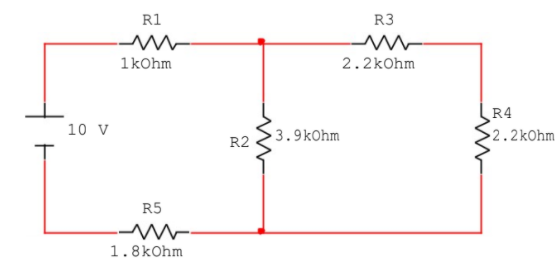
\includegraphics[scale=0.55]{Informe/Circuito Resistivo Mixto.png}
\label{Fig.1}
\caption {Circuito Resistivo Mixto}
\end{figure}

\clearpage

\section{Procedimiento}
1.Arme el circuito que se muestra en la figura \ref{Fig.1}\\

2.Mida el voltaje y corriente en cada uno de los elementos del circuito. Anote los resultados de las mediciones en la tabla \ref{tab.1}
\begin{table}[h]
\caption{\label{tab.1}
Resultados obtenidos de voltaje y corriente, en cada elemento del circuito.}
\begin{ruledtabular}
\begin{tabular}{Tabla de datos}
 $Variable$&$Valor Calculado$&$Valor Medido$\\
\hline
V_{r1}(V)& 2.05 & 2.054\\
I_{r1}(mA)& 2.05 & 2.05\\
V_{r2}(V)& 4.22 & 4.247\\
I_{r2}(mA)& 1.08 & 1.08\\
V_{r3}(V)& 2.09 & 2.12\\
I_{r3}(mA)& 0.95 & 0.965\\
V_{r4}(V)& 2.09 & 2.12\\
I_{r4}(mA)& 0.95 & 0.965\\
V_{r5}(V)& 3.69 & 3.69\\
I_{r5}(mA)& 2.05 & 2.054\\
\end{tabular}
\end{ruledtabular}
\end{table}\\  

3.Verifique si se cumple la Ley de Kirchhoff de Voltajes en cada trayectoria cerrada, considerando las elevaciones de voltaje con signo positivo y las caídas de voltaje con signo negativo. Anote los resultados en la \ref{tab.2}
\begin{table}[h]
\caption{\label{tab.2}
Resultados obtenidos de voltaje y corriente, en cada elemento del circuito.}
\begin{ruledtabular}
\begin{tabular}{Tabla de datos}
 $Voltaje$&$Trayectoria 1$& &$Trayectoria 2$\\
 $ $&$Calculado$&$Medido$&$Calculado$&$Medido$\\
\hline
V_T(V)& 2.053 & 2.05 & 4.24 & 4.24\\
V_{r1}(V)& 2.053 & 2.054 &  & \\
V_{r2}(V)& 4.24 & 4.247 & 4.24 & 4.247\\
V_{r3}(V)&  &  & 2.12 & 2.12\\
V_{r4}(V)&  &  & 2.12 & 2.12\\
V_{r5}(V)& 3.69 & 3.69 &  & \\
V(V)& 12.03 & 12.041 & 12.72 & 12.727\\
\verb+%+Error& 0.091\verb+%+ & & 0.055\verb+%+\\
\end{tabular}
\end{ruledtabular}
\end{table}\\ 

4.Verifique si se cumple la Ley de Kirchhoff de Corrientes en cada nodo, tomando con signo positivo las corrientes que entran al nodo y con signo negativo las que salen del nodo. Anote los resultados en la tabla \ref{tab.3}
\begin{table}[h]
\caption{\label{tab.3}
Resultados obtenidos de voltaje y corriente, en cada elemento del circuito.}
\begin{ruledtabular}
\begin{tabular}{Tabla de datos}
 $Corriente$&$Maya 1$& &$Mata 2$\\
 $ $&$Calculado$&$Medido$&$Calculado$&$Medido$\\
\hline
I_T(mA)& 2.053 & 2.05 & 0.965 & 0.965\\
I_{r1}(mA)& 2.053 & 2.05 &  & \\
I_{r2}(mA)& 2.053 & 2.05 & 0.965 & 0.965\\
I_{r3}(mA)&  &  & 0.965 & 0.965\\
I_{r4}(mA)&  &  & 0.965 & 0.965\\
I_{r5}(mA)& 2.053 & 2.054 &  & \\
I(mA)& 8.212 & 8.8216 &  & \\
\verb+%+Error& 0.048\verb+%+ & & 0\verb+%+\\
\end{tabular}
\end{ruledtabular}
\end{table}\\

5.Compare los resultados medidos con los valores obtenidos al analizar el circuito analíticamente y concluya al respecto.\\ 

\subsection{Resultados}

Maya 1

\begin{array}
    &10+1kI_1-3.9k(I_1-I_2)-1.8kI_2=0 
\\ 10-6.7kI_1+3.9kI_2=0 
\\ 6.7I_1-3.9I_2=10(1)
\end{array}\\

Maya 2

\begin{array}
    &-2.2kI_2-2.2kI_2-3.9k(I_2-I_1)=0
\\ -8.3kI_2+3.9kI_2=0 (2)
\end{array}\\

Sistema de Ecuaciones con (1) y (2)

\left.
\begin{array}{rcl}
    6.7I_1-3.9I_2=10 
\\ 3.9I_1-8.3I_2=0
\end{array}\\
\right\}

Resolviendo:

\begin{array}
    I_1=2.053 mA & & $Esta es la corriente que circula en la primera maya$
\\I_2=0.965 mA & & $ Esta es la corriente que circula en la segunda maya$
\end{array}\\

Para encontrar los voltajes ocupamos la ley de Ohm

\begin{array}
    &V=I*R
\\VR_1=2.053mA*1K
\\VR_1=2.053 V
\end{array}\\

Para encontrar el voltaje en la resistencia 2 debemos hacer una diferencia entre la corriente 1 y la corriente 2

\begin{array}
    &IR_2=I_1-I_2
\\IR_2=2.053 mA-0.965 mA
\\IR_2=1.088 mA
\\VR_2=1.088 mA*3.9K
\\VR_2=4.24V
\\VR_3=0.965 mA*2.2K
\\VR_3=2.12V
\\VR_4=0.965 mA*2.2K
\\VR_4=2.12V
\\VR_5=2.053mA*1.8k
\\VR_5=3.69V
\end{array}\\

Para poder calcular el error debemos aplicar la siguiente formula:\\

$Error=\frac{v_{teórico}-v_{medido}}{v_{teórico}}100\verb+%+$ 

\section{Descripción de prerrequisitos y configuración}

\begin{itemize}
    \item Tinkercad: Es una herramienta online de Autodesk, que permite la simulación de circuitos, al igual que permite dibujar esquemas circuitales de forma sencilla.
    \item LTspice: Es un simulador de alto rendimiento en el que pueden armarse diagramas esquemáticos de reguladores de alimentación conmutados o Convertidores DC-DC. Permite la simulación de circuitos.
\end{itemize}

\section{Conclusiones}

\verb+Conclusiones+ \\

- La leyes de Kirchhoff nos ayudan en el análisis de circuitos eléctricos, como el empleado en la practica, lo cual hace que sea un método muy utilizado en el análisis de valor de voltaje o corriente.\\

- Los valores medidos no se alteran mucho a los valores teóricos, por lo cual nuestro valor de error en la practica no es tan alto.\\

\section{Anexos}
\begin{figure}[h]
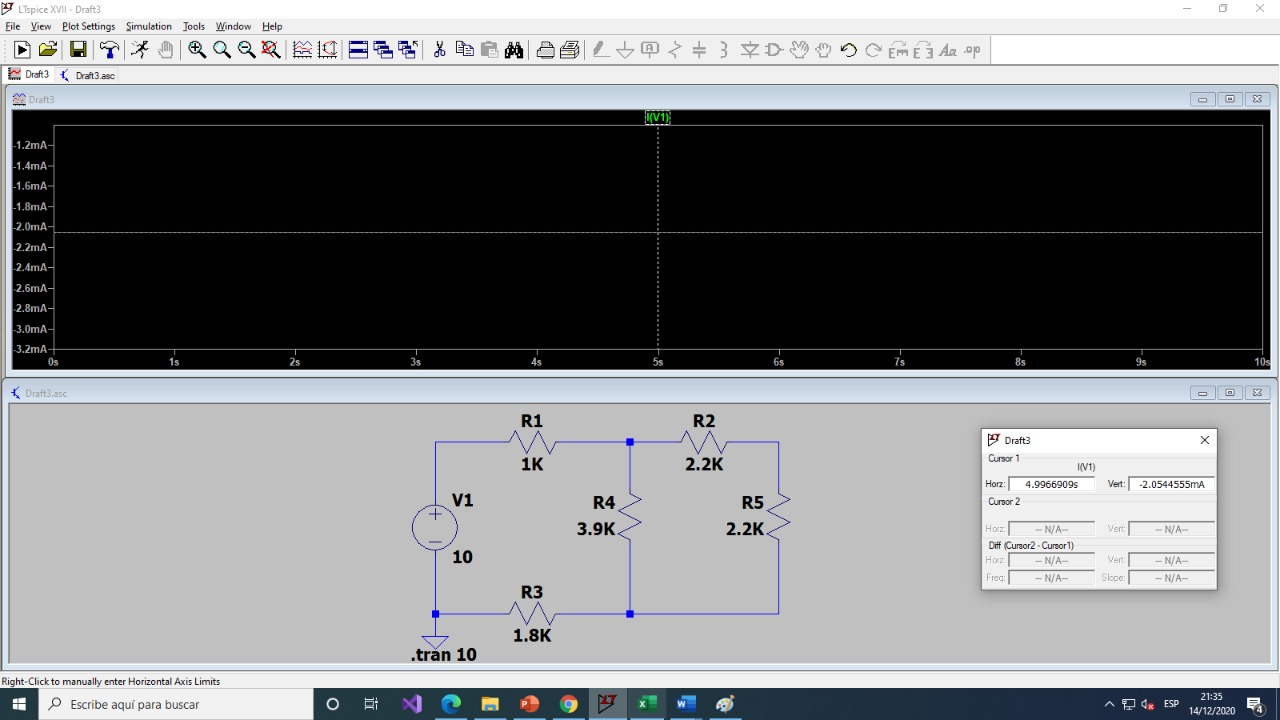
\includegraphics[scale=0.2]{Informe/Circuito en LTspice.jpeg}
\caption{Circuito en LTspice}
\end{figure}
\begin{figure}[h]
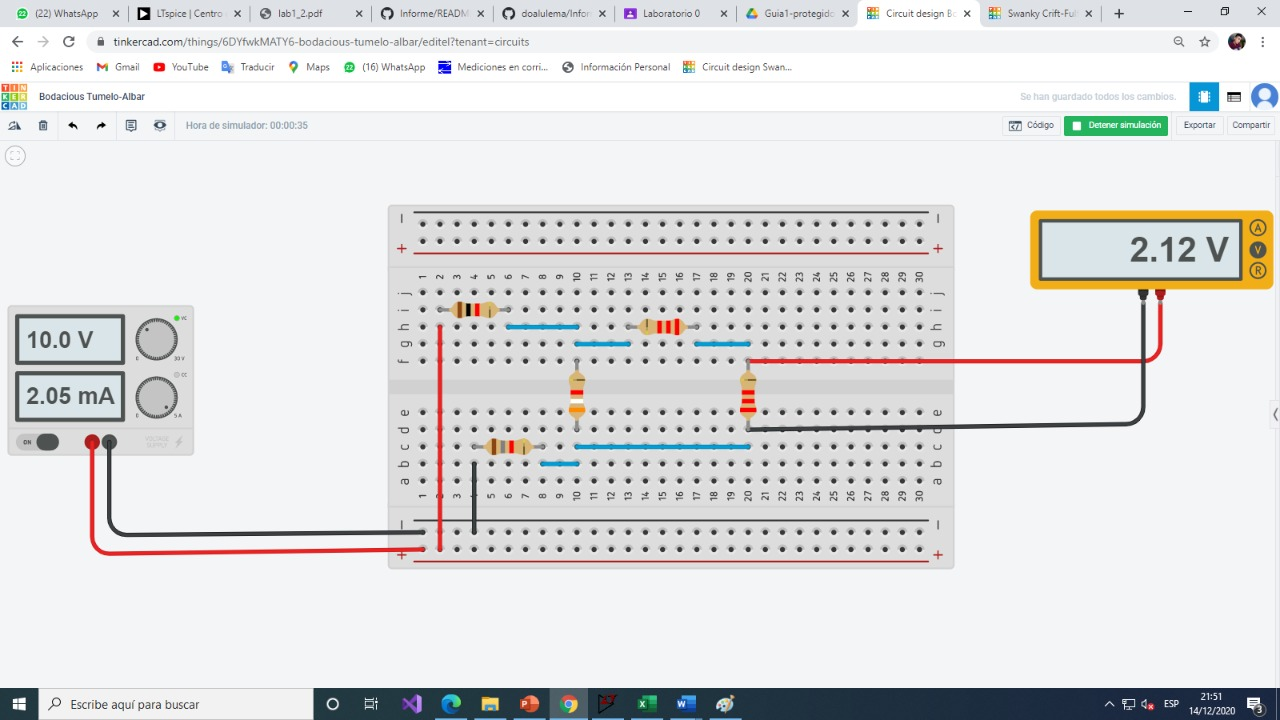
\includegraphics[scale=0.2]{Informe/Circuito en Tinkercad1.jpeg}
\caption{Circuito en Tinkercad1}
\end{figure}
\begin{figure}[h]
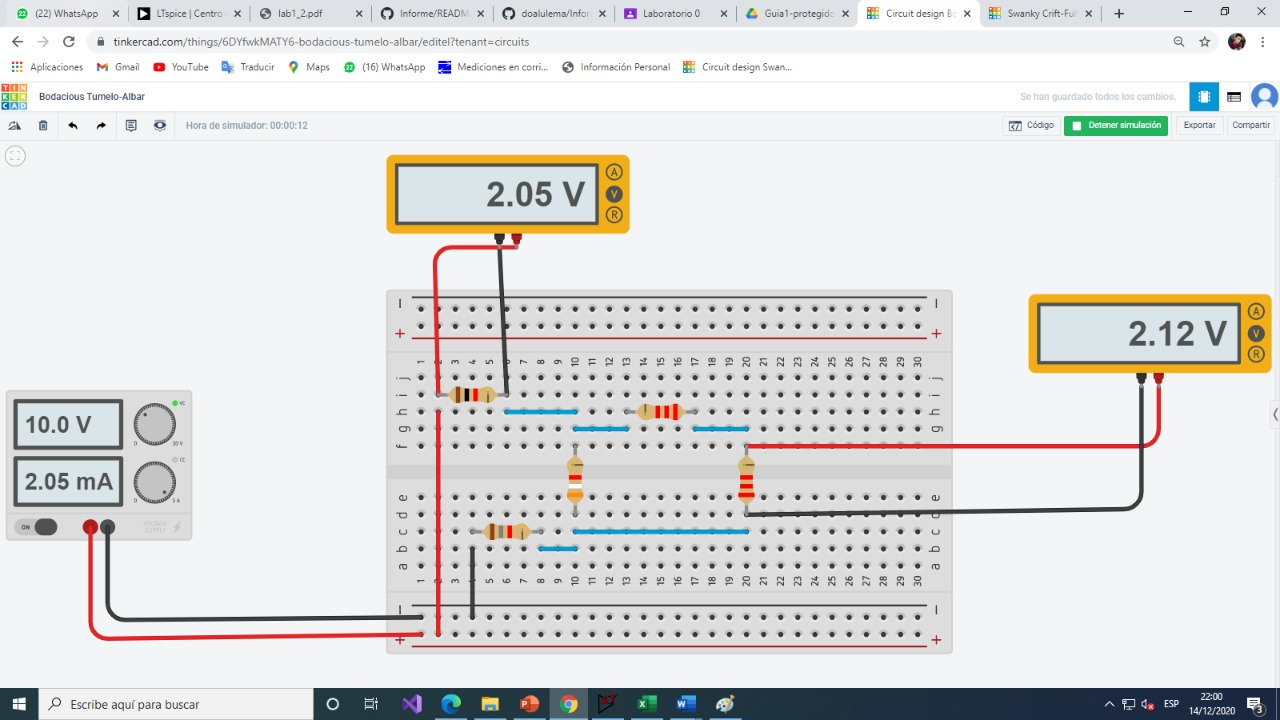
\includegraphics[scale=0.2]{Informe/Circuito en Tinkercad2.jpeg}
\caption{Circuito en Tinkercad2}
\end{figure}
\clearpage
\printbibliography[h]

\end{document}